\chapter{Einleitung}\label{introduction}
Die Medienlandschaft hat sich durch das das Internet stark verändert. Die früher dominierenden Printmedien mussten und müssen mit sinkenden Einnahmen leben und so wird es immer wichtige eine starke und aktuelle Onlinepräsenz zu haben. Damit wird Werbung als Einnahmequelle immer wichtiger. Da Werbung inzwischen einer der wichtigsten Einnahmequellen für viele Internetpublisher ist, sind Besucherzahlen entscheidend.
In den vergangenen Jahren hat sich eine Form von Content entwickelt(oder wurde vielmehr wiederentdeckt) die gemeinhin als Clickbait bezeichnet wird.
Bei diesen wird durch möglichst reißerische, emotionale und offen gestaltete Überschriften versucht, den Nutzer von Plattformen von Twitter, Facebook und Ähnlichem zum Besuchen zu ``überreden''.  Durch die Verbreitung in sozialen Medien, und der durch viele empfundene Zwang, Artikel mit dieser Form von Überschrift zu lesen, hat Clickbait viele Feinde gemacht, doch die Effektivität dieser Methoden steht außer Frage. Im Rahmen dieser Bachelor Arbeit wurden aus Mangel an Fach-Literatur aber auch um den ... darzustellen einige hundert Clickbait verwandte Blog Einträge ausgewertet und die Meinung der Blogger ist klar: Clickbait ist irreführend, sensationalistisch und enttäuschend. 
%https://archive.is/Dxdl2

Um Clickbait zu beschreiben wurden in \cite{paper:clickbait-detection2} die Begriffe \textquote{Message} und \textquote{Target} eingeführt. Dabei beschreibt die Message den Teil, der auf den Hauptcontent, das Target, verweist, im Falle Twitter der entsprechende Tweet --Bild---, er hat den Auftrag den Leser zum Click auf den Link zu bewegen.

Daraus ergibt sich das Thema dieser Arbeit: wie gut können wir Clickbait mit Hilfe von Machine Learning erkennen? 
Denkbare Funktionen dieser Erkennung wäre ein Einsatz in Form eines Spamfilters, der den jeweiligen NewsFeed auf relevante Bereiche und Nachrichten beschränkt und Menschen hilft sich nicht ablenken zu lassen.

Auf Clickbait, seine Formen und Ausprägungen wird genauer in Kapitel~\ref{cha:clickbait} eingegangen.

Um Clickbait erkennen zu können wird ein annotierter Korpus benötigt, mit welchen Klassifikatoren trainiert werden können. Da kein relevanter Korpus gefunden wurde, ergab sich die Notwenigkeit diesen selbst zu sammeln und zu annotieren.
Dazu haben wir 3000 Tweets der 25 größten  Newspublisher  auf Twitter gesammelt und anschließend annotiert. Auf die Corpuserstellung und Annotation wird in Kapitel~\ref{cha:korpus} genau eingegangen.
Auf dem nun erstellten Korpus konnten nun das Machine-Learning ausgeführt werden. Dazu wurden neben den herkömmlichen Bag-of-Word Features eine vielzahl ein weiterer Features Verwendet, welche sich grob in die Kategorien
\begin{itemize}
  \item Message-Features: Hier wird die Message selbst in einer Reihe von Features dargestellt, unter anderem als Bag-of-Words und die Flesch-Reading-Ease
  \item Target-Features: Hier wird das Target der Message dargestellt, mit ähnlichen Features wie die Message selbst
  \item Meta-Features: Hierbei werden Metainformationen der Message betrachtet, zum Beispiel der User, welcher die Message verfasst hat
\end{itemize}
unterteilen lassen. Die Details werden in Kapitel~\ref{cha:maschine_learning} beschrieben.
Im Folgenden Kapitel~\ref{cha:auswertung} wird auf die Ergebnisse dieser Experimente eingegangen.
Um den Ergebnisse zu visualisieren und praktisch testen zu können wurde ein Webservice erstellt, bei dem man die Klassifizierung der trainierten Klassifizierer an aktuellen Tweets betrachten kann. Der Aufbau und die Funktion dieses Webservices werden in Kapitel~\ref{webservice} beschrieben.
Anschließend werden in Kapitel~\ref{cha:conclusion} Ergebnisse noch einmal zusammengefasst, und ein Ausblick auf zukünftige mögliche Aufgaben der Forschung gegeben.



Überschrift muss aus großer auswahl hervorstechen


In \enquote{Content Analysis of Magazine Headlines: Changes over Three Decades?} \cite{davalos2007iii} wird der Frage nachgegangen, inwiefern sich die Überschriften von Magazinen, besonders an Frauen gerichtete, innerhalb von 30 Jahren verändert haben.
\begin{figure}
\label{tab:womenclickbait}
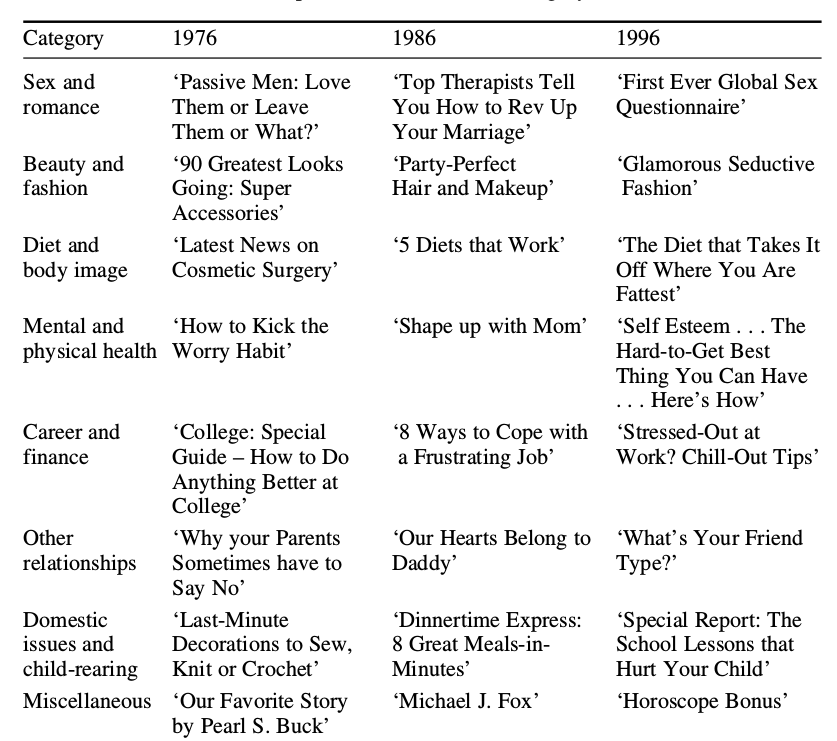
\includegraphics[width=0.5\textwidth]{../images/women-magazine-clickbait}
\end{figure}\todo{hübsch machen}
Bei dem in Darstellung~\ref{tab:womenclickbait} gezeigten Überschriften zeigt sich, das
1976 Überschriften verwendet wurden, die 


